\chapter{Cluster Analysys}
\label{ch:cluster}

    In questo capitolo si descriveranno le attività svolte per realizzare dei \textit{clustering} sulle versioni ad attributi continui dei data set prodotti nella fase di \textit{preprocessing} (descritta nel Capitolo \ref{ch:prepr}).

\section{Introduzione alla Cluster Analysys}

    Impiegando una massiccia astrazione dai dettagli, possiamo descrivere un \textit{clustering} come segue, riportandolo direttamente da \cite{clustering}:\\

    "Il \textbf{clustering} o \textbf{analisi dei gruppi} (dal termine inglese \textit{cluster analysis} introdotto da Robert Tryon nel 1939) è un insieme di tecniche di analisi multivariata dei dati volte alla selezione e raggruppamento di elementi omogenei in un insieme di dati."\\

    Volendo sintetizzare ulteriormente questi concetti, si può dire che un \textit{clustering} su di un certo data set è un raggruppamento di istanze \textbf{simili fra loro}. Citando sempre da \cite{clustering}:\\

    "Le tecniche di clustering si basano su misure relative alla somiglianza tra gli elementi. In molti approcci questa similarità, o meglio, dissimilarità, è concepita in termini di distanza in uno spazio multidimensionale. La bontà delle analisi ottenute dagli algoritmi di clustering dipende molto dalla scelta della metrica, e quindi da come è calcolata la distanza. Gli algoritmi di clustering raggruppano gli elementi sulla base della loro distanza reciproca, e quindi l'appartenenza o meno ad un insieme dipende da quanto l'elemento preso in esame è distante dall'insieme stesso."\\

    La similitudine fra due istanze si intende quindi come una misura di \textbf{distanza} in uno spazio multidimensionale le cui dimensioni sono gli attributi delle istanze stesse.\\

    Questo scritto può essere sufficiente per delineare il quadro generale nel quale si è operato per compiere i passi descritti successivamente. Ovviamente, una trattazione esaustiva sull'argomento necessiterebbe ben altro spazio di quello che si può dedicare in questa tesi di laurea, perciò si rimanda alla consultazione di \cite{dispense} per ulteriori dettagli, qualora quanto sopra riportato non dovesse essere sufficiente per la comprensione di quanto seguirà.

\section{Algoritmi di Clustering}

    La realizzazione di un \textit{clustering} su dei \textit{big data} è ovviamente una di quelle attività che hanno bisogno di essere delegate a un algoritmo per essere eseguite. Si descriveranno in questa sezione alcuni dei più efficaci algoritmi di \textit{clustering} e le implementazioni di Weka.

    \subsection{Algoritmo K-Means}

        Uno dei più noti algoritmi di \textit{clustering} che consente di imporre a priori il numero di \textit{cluster} cercati è senza dubbio \textbf{K-Means}. Come si può leggere in \cite{dispense}:\\

        "The K-means clustering technique is simple [...]. We first choose \textit{K} initial centroids, where \textit{K} is a user-specified parameter, namely, the number of clusters desired. Each point is then assigned to the closest centroid, and each collection of points assigned to a centroid is a cluster. The centroid of each cluster is then updated based on the points assigned to the cluster. We repeat the assignment and update steps until no point changes clusters, or equivalently, until the centroids remain the same." \\

        Il che significa, traducendo e parafrasando:\\

        "La tecnica K-Means è semplice: scegliamo inizialmente \textit{K} centroidi iniziali, dove \textit{K} è il numero di cluster desiderati. Ogni punto del data set è assegnato al centroide più vicino, e ogni collezione di punti assegnati a un centrode è un cluster. Il centroide di ogni cluster viene poi ricalcolato, basandosi sui punti che gli sono stati assegnati. Si ripetono questi passi fino a che nessun punto cambia cluster, o i centroidi non cambiano."\\

        Quindi, si tratta di una procedura iterativa che, a partire da un numero fissato di centroidi iniziali, migliora ad ogni passo gli assegnamenti fino a che non si raggiunge una situazione di stabilità. \\

        Le librerie di Weka mettono a disposizione una implementazione di K-Means, che offre di poter configurare un gran numero di parametri (come si può vedere in Figura \ref{kmeans_weka}).

        \begin{figure}
            \centering
            \caption{finestra che mostra i parametri impostabili dell'algoritmo K-Means}
            \label{kmeans_weka}
            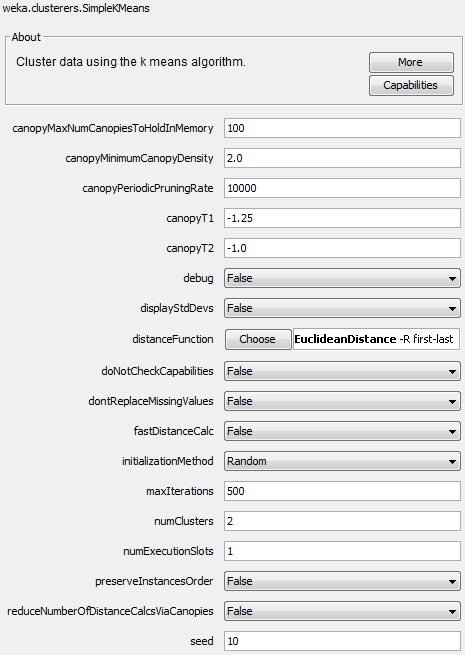
\includegraphics[scale=0.55]{img/cluster_k_means.png}
        \end{figure}

    \subsection{Algoritmo DBSCAN di Weka}
        Lorem ecc

        \begin{figure}
            \centering
            \caption{finestra che mostra i parametri impostabili dell'algoritmo DBSCAN}
            \label{dbscan_weka}
            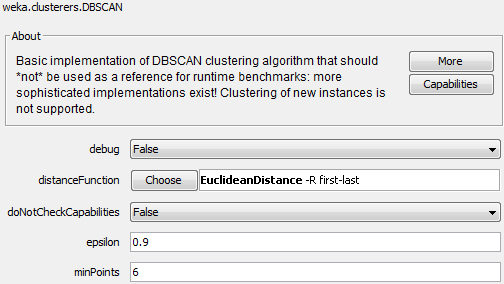
\includegraphics[scale=0.50]{img/dbscan_weka.png}
        \end{figure}

    \subsection{Algoritmo di Clustering Gerarchico}

        \begin{figure}
            \centering
            \caption{finestra che mostra i parametri impostabili dell'algoritmo di clustering gerarchico}
            \label{hierar_weka}
            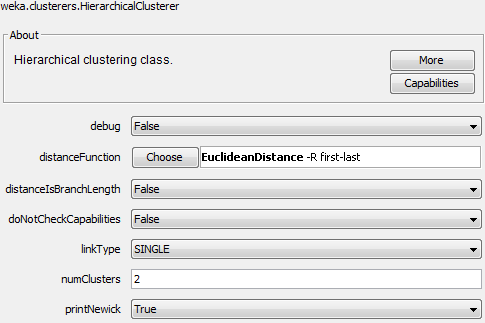
\includegraphics[scale=0.50]{img/hierarch_weka.png}
        \end{figure}

\section{Clustering sulle Valutazioni dei Corsi}

    \subsection{Lancio di K-Means e analisi dei risultati}

    \subsection{Tentativo di utilizzo di DBSCAN}

\section{Clustering sulla Produttività degli Studenti}

    ...

    \subsection{Clustering Gerarchico}

\section{Clustering sulla join dei due data set}

    \subsection{Lancio di $K-Means$}

    \subsection{Analisi dei risultati di $K-Means$}